% Merged method figure, candidate A: three columns read left to right, each read top to bottom.
%   (a) concept: AReA's one schedule above SCA's 1,368 per-head weights, shared sigma axis (../method_v2/cloud_a.png)
%   (b) calibrate once at 1024^2: full attention on the real calibration image ~ pi_h local + (1 - pi_h) global
%       at ratio r = 4 (to scale on the 64 x 64 grid), closed form, the table cards (ratios 2 and 4)
%   (c) sample progressively: noise, 1024^2 full, 2048^2 and 4096^2 SCA stages, the real progressive output; the
%       mix of an SCA stage as a zoomed inset fed by the table
% Build from this directory:  ~/.local/bin/tectonic --outdir .. method_v2a.tex   (writes ../method_v2a.pdf)
% Print size: 1 unit = 1 pt, canvas 397.48 pt (5.5 in) wide. Text: titles 8.5 pt bold sans, labels 7.5 pt,
% ticks and sizes 7 pt, math 8 pt (scripts 6 pt). Data: ../method_v2/ (fig_method_v2.py, provenance.json).
\documentclass[border=0pt]{standalone}
\RequirePackage{fix-cm}
\usepackage[T1]{fontenc}
\usepackage{helvet}
\usepackage{amsmath}
\usepackage{graphicx}
\usepackage{tikz}
\usetikzlibrary{arrows.meta, calc}
\DeclareMathSizes{7}{7}{6}{6}
\DeclareMathSizes{7.5}{7.5}{6}{6}
\DeclareMathSizes{8}{8}{6.2}{6}
\DeclareMathSizes{8.5}{8.5}{6.5}{6}
\DeclareMathSizes{10}{10}{7}{6}
% Written by scafig.py; the same palette as the matplotlib figures.
\definecolor{scaInk}{HTML}{1F2328}
\definecolor{scaMid}{HTML}{5B6570}
\definecolor{scaRule}{HTML}{C3C9CF}
\definecolor{scaGrid}{HTML}{E6E9EC}
\definecolor{scaGlobal}{HTML}{2F6DB3}
\definecolor{scaGlobalLight}{HTML}{DCE7F3}
\definecolor{scaLocal}{HTML}{E08A2B}
\definecolor{scaLocalLight}{HTML}{F9E6D0}
\definecolor{scaAccent}{HTML}{13865F}
\definecolor{scaAccentLight}{HTML}{D7EEE4}
\definecolor{scaNeutral}{HTML}{F4F1EA}
\definecolor{scaZoom}{HTML}{FFC21A}
\definecolor{scaLoss}{HTML}{B85C00}
\definecolor{scaArea}{HTML}{7A4EA3}
\definecolor{scaAreaLight}{HTML}{E9E0F1}
\definecolor{scaFull}{HTML}{9AA3AC}
\definecolor{scaCrop}{HTML}{E4572E}

% Written by fig_method_v2.py from results/heads_view/concept_curves.csv; do not edit by hand.
\def\CvXL{1.00}\def\CvXR{0.10}\def\CvYL{-0.06}\def\CvYH{1.06}
\def\CvGate{0.89}
\def\NHeads{1{,}368}
\expandafter\def\csname CvWa\endcsname{84.0}\expandafter\def\csname CvHa\endcsname{56.0}
\expandafter\def\csname CvWb\endcsname{170.0}\expandafter\def\csname CvHb\endcsname{38.0}

\definecolor{scaLocalText}{HTML}{A85F12}
\definecolor{scaGlobalText}{HTML}{245A96}

\newcommand{\ttl}{\fontsize{9}{10.5}\selectfont\sffamily\bfseries}
\newcommand{\lab}{\fontsize{7.5}{9}\selectfont\sffamily}
\newcommand{\sml}{\fontsize{7}{8}\selectfont\sffamily}
\newcommand{\mth}{\fontsize{8}{9.5}\selectfont}
\newcommand{\mts}{\fontsize{7}{8}\selectfont}
\newcommand{\bigsym}{\fontsize{10}{12}\selectfont}

\tikzset{
  every node/.style={inner sep=0pt, outer sep=0pt, text=scaInk},
  arr/.style={-{Stealth[length=3.2pt, width=2.8pt]}, line width=0.6pt, draw=scaInk},
  blk/.style={rounded corners=2pt, line width=0.8pt},
  sblk/.style={blk, draw=scaAccent, fill=scaAccentLight},
  nblk/.style={blk, draw=scaFull, fill=white},
  axis/.style={line width=0.5pt, draw=scaMid},
  zoom/.style={line width=0.5pt, draw=scaAccent, dash pattern=on 1.5pt off 1.2pt},
}

% ---------------------------------------------------------------- curve plots
\newcommand{\SX}[3]{#1+#3*(\CvXL-#2)/(\CvXL-\CvXR)}     % \SX{x0}{sigma}{w}
\newcommand{\PY}[3]{#1+#3*(#2-\CvYL)/(\CvYH-\CvYL)}     % \PY{y0}{pi}{h}
\newcommand{\Axes}[6]{% x0 y0 w h ylabels(0/1) xlabels(0/1)
  \draw[axis] (#1,#2) rectangle ++(#3,#4);
  \foreach \s/\t in {1/1, 0.89/{}, 0.5/0.5, 0.1/0.1}{
    \draw[axis] ({\SX{#1}{\s}{#3}},#2) -- ++(0,-1.6);
    \ifnum#6=1 \node[anchor=north, text=scaMid] at ({\SX{#1}{\s}{#3}},#2-2.4) {\sml\t};\fi}
  \foreach \v in {0,1}{\draw[axis] (#1,{\PY{#2}{\v}{#4}}) -- ++(-1.6,0);}
  \ifnum#5=1
    \foreach \v in {0,1}{\node[anchor=east, text=scaMid] at (#1-2.4,{\PY{#2}{\v}{#4}}) {\sml\v};}
  \fi}

% ---------------------------------------------------------------- calibration image tiles at r = 4
% Token geometry on the 64 x 64 grid (row 0 at the top): window rows 19..34, cols 23..38 (16 x 16, centred on the
% 2 x 2 query tile at rows 26..27, cols 30..31, drawn enlarged to 4 x 4); block centres at 4b + 2, b = 0..15.
\newcommand{\Query}[1]{%
  \fill[scaInk] (29*#1/64,{#1-29*#1/64}) rectangle (33*#1/64,{#1-25*#1/64});
  \draw[white, line width=0.35pt] (29*#1/64,{#1-29*#1/64}) rectangle (33*#1/64,{#1-25*#1/64});}
\newcommand{\CalTile}[4]{% x y side mode(0 full, 1 local, 2 global)
  \begin{scope}[shift={(#1,#2)}]
    \node[anchor=south west] at (0,0) {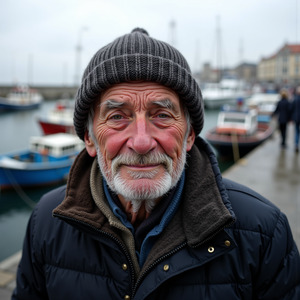
\includegraphics[width=#3pt]{../method_flow/calib.jpg}};
    \ifcase#4
      \draw[line width=0.6pt, scaFull] (0,0) rectangle (#3,#3);
    \or
      \fill[white, opacity=0.7, even odd rule] (0,0) rectangle (#3,#3)
        (23*#3/64,{#3-35*#3/64}) rectangle (39*#3/64,{#3-19*#3/64});
      \draw[line width=0.6pt, scaFull] (0,0) rectangle (#3,#3);
      \draw[line width=0.9pt, scaLocal] (23*#3/64,{#3-35*#3/64}) rectangle (39*#3/64,{#3-19*#3/64});
    \or
      \fill[white, opacity=0.62] (0,0) rectangle (#3,#3);
      \draw[line width=0.6pt, scaFull] (0,0) rectangle (#3,#3);
      \foreach \i in {0,...,15}{\foreach \j in {0,...,15}{
        \fill[scaGlobal] ({(4*\i+2.5)*#3/64},{#3-(4*\j+2.5)*#3/64}) circle[radius=0.42pt];}}
    \fi
    \Query{#3}
  \end{scope}}

% ---------------------------------------------------------------- schematic views at a target stage
\newcommand{\Tile}[1]{\fill[scaGrid] (0,0) rectangle (#1,#1); \draw[line width=0.5pt, scaFull] (0,0) rectangle (#1,#1);}
\newcommand{\QueryC}[1]{\fill[scaInk] ({0.47*#1},{0.53*#1}) rectangle ++({0.07*#1},{0.07*#1});
  \draw[white, line width=0.3pt] ({0.47*#1},{0.53*#1}) rectangle ++({0.07*#1},{0.07*#1});}
\newcommand{\LocIcon}[4]{\begin{scope}[shift={(#1,#2)}]\Tile{#3}
  \pgfmathsetmacro{\wh}{0.5*#3/#4}
  \fill[scaLocalLight] ({0.505*#3-\wh},{0.565*#3-\wh}) rectangle ({0.505*#3+\wh},{0.565*#3+\wh});
  \draw[scaLocal, line width=0.8pt] ({0.505*#3-\wh},{0.565*#3-\wh}) rectangle ({0.505*#3+\wh},{0.565*#3+\wh});
  \QueryC{#3}\end{scope}}
\newcommand{\GlobIcon}[4]{\begin{scope}[shift={(#1,#2)}]\Tile{#3}
  \foreach \i in {0,...,11}{\foreach \j in {0,...,11}{\fill[scaGlobal] ({(\i+0.5)*#3/12},{(\j+0.5)*#3/12}) circle[radius=0.42pt];}}
  \QueryC{#3}\end{scope}}
% schematic stage tile: side #3, label #4 inside, style #5
\newcommand{\Stage}[5]{\draw[#5] (#1,#2) rectangle ++(#3,#3); \node at ({#1+0.5*#3},{#2+0.5*#3}) {#4};}

\begin{document}
\begin{tikzpicture}[x=1pt, y=1pt]
\useasboundingbox (0,0) rectangle (397.48,180);

% ================================================================== (a) concept, x 0..104
\node[anchor=north west] at (0,179) {\ttl (a) One weight per head};
\def\ax{18}\def\aw{\CvWa}\def\ah{\CvHa}
% AReA: one schedule, every head
\def\ay{94}
\Axes{\ax}{\ay}{\aw}{\ah}{1}{0}
\draw[line width=1.3pt, scaArea, line cap=round, line join=round]
  ({\SX{\ax}{1}{\aw}},{\PY{\ay}{0}{\ah}}) -- ({\SX{\ax}{\CvGate}{\aw}},{\PY{\ay}{0}{\ah}})
  -- ({\SX{\ax}{\CvGate}{\aw}},{\PY{\ay}{1}{\ah}}) -- ({\SX{\ax}{0.1}{\aw}},{\PY{\ay}{1}{\ah}});
\node[anchor=base east, text=scaArea] at (\ax+\aw,{\ay+\ah+3.4}) {\lab AReA: every head};
% SCA: one weight per head, same axes
\def\by{17}
\node[anchor=south west] at (\ax,\by) {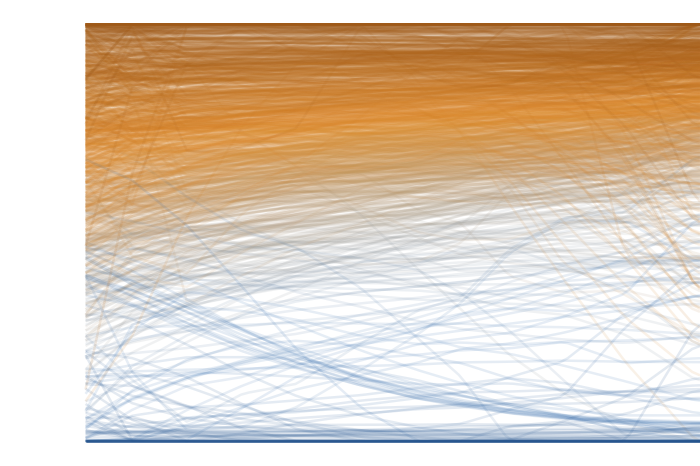
\includegraphics[width=\aw pt, height=\ah pt]{../method_v2/cloud_a.png}};
\Axes{\ax}{\by}{\aw}{\ah}{1}{1}
\node[anchor=base east, text=scaAccent] at (\ax+\aw,{\by+\ah+3.4}) {\lab SCA: each of \NHeads{} heads};
\node at (6,{\by+0.5*\ah}) {\mth $\pi_h$};
\node at (6,{\ay+0.5*\ah}) {\mth $\pi_h$};
\node[anchor=north east, text=scaMid] at (\ax-4,\by-2.4) {\mth $\sigma$};

% ================================================================== (b) calibrate once at 1024^2, x 116..236
\node[anchor=north west] at (116,179) {\ttl (b) Calibrate once at 1024\textsuperscript{2}};
\CalTile{154}{122}{44}{0}
\node[anchor=west, align=left, font=\lab] at (201,144) {full\\attention};
\node at (176,113) {\bigsym $\approx$};
\def\ry{72}\def\rs{30}
\node[anchor=west] at (116,{\ry+0.5*\rs}) {\mth $\pi_h$};
\CalTile{128}{\ry}{\rs}{1}
\node at (163,{\ry+0.5*\rs}) {\mth $+$};
\node at (185,{\ry+0.5*\rs}) {\mth $(1-\pi_h)$};
\CalTile{204}{\ry}{\rs}{2}
\node[anchor=north, text=scaLocalText] at (143,\ry-2) {\lab local};
\node[anchor=north, text=scaGlobalText] at (219,\ry-2) {\lab global};
\node[anchor=south east, text=scaMid] at (234,\ry+\rs+1.5) {\mts $r=4$};
% closed form on the edge, then the table cards (one block, 24 heads x 13 noise bins; ratio 2 behind, 4 in front)
\draw[line width=0.6pt, scaInk] (176,61) -- (176,56.5);
\node[fill=white, inner xsep=1pt, inner ysep=1pt] at (176,51) {\mth $\pi_h^\star=\mathrm{clip}(B/A)$};
\draw[arr] (176,45.5) -- (176,37.4);
\node[anchor=south west] at (165,8) {
\includegraphics[width=32pt, height=26pt]{../method_v2/table_r2.png}};
\draw[line width=0.5pt, scaFull] (165,8) rectangle ++(32,26);
\fill[white] (160,3) rectangle ++(32,26);
\node[anchor=south west] at (160,3) {
\includegraphics[width=32pt, height=26pt]{../method_v2/table_r4.png}};
\draw[line width=0.5pt, scaFull] (160,3) rectangle ++(32,26);
\node[anchor=west] at (201,18) {\mth $\pi_h(\sigma,r)$};

% ================================================================== (c) sample progressively, x 248..397
\node[anchor=north west] at (248,179) {\ttl (c) Sample progressively};
% the stage chain runs down the right of the column, centred on x = 365; tiles hold their size
\def\cx{365}
\node at (\cx,157) {
\includegraphics[width=16pt]{../method_flow/noise.png}};
\draw[arr] (\cx,148.6) -- (\cx,142.4);
\Stage{\cx-12}{119}{24}{\sml 1024\textsuperscript{2}}{nblk}
\node[anchor=west] at (\cx+15,131) {\sml full};
\draw[arr] (\cx,118.2) -- (\cx,109.6);
\node[anchor=east, text=scaMid] at (\cx-3,114) {\mts $\times2$};
\Stage{\cx-12}{85}{24}{\sml 2048\textsuperscript{2}}{sblk}
\node[anchor=west] at (\cx+15,97) {\mts $r{=}2$};
\draw[arr] (\cx,84.2) -- (\cx,76.6);
\node[anchor=east, text=scaMid] at (\cx-3,80.5) {\mts $\times2$};
\Stage{\cx-12}{51}{24}{\sml 4096\textsuperscript{2}}{sblk}
\node[anchor=west] at (\cx+15,63) {\mts $r{=}4$};
\draw[arr] (\cx,50.2) -- (\cx,45.4);
\node[anchor=north] at (\cx,44.6) {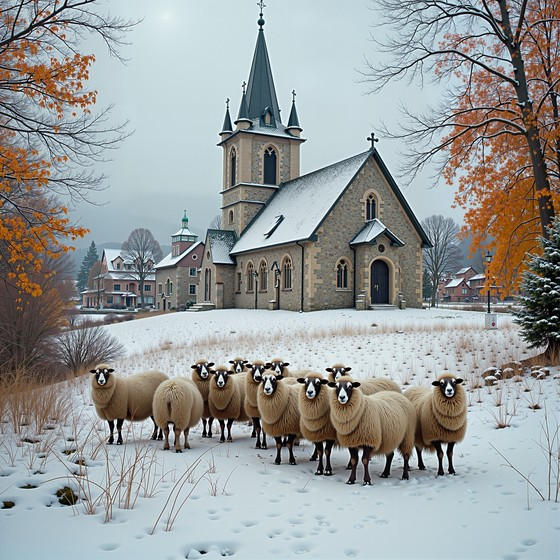
\includegraphics[width=43pt]{../method_flow/output_prog.jpg}};
% inset: the mix inside every SCA stage, a pale wedge from the SCA tiles
\fill[scaAccentLight!70] (353,52) -- (353,108) -- (336,116) -- (336,46) -- cycle;
\draw[sblk] (256,46) rectangle (336,116);
\node[anchor=east] at (299,97) {\mth $\pi_h$};
\LocIcon{302}{84}{26}{4}
\node at (315,78.5) {\mth $+$};
\node[anchor=east] at (299,59) {\mth $(1-\pi_h)$};
\GlobIcon{302}{50}{26}{4}
% the table feeds the mix
\draw[arr] (197,13) -- (246,13) -- (246,81) -- (255.2,81);
\end{tikzpicture}
\end{document}
